\documentclass[titlepage, 10pt]{article}

\usepackage{graphicx} %[pdftex]
\usepackage[hidelinks]{hyperref}
\usepackage{titlepic}
\usepackage{fullpage}
\usepackage{pdfpages}
\usepackage[lined,ruled]{algorithm2e}

\titlepic{
\includegraphics[width=0.30\textwidth]{img/sedes.jpg}}
\title
{
	[H03I7A] Design in Medical Technology\\
	Shape-based feature analysis\\
	for nodule detection in lung images
}
\author{Kim Nuyts \and Sven Van Hove}
\date{\today}

\begin{document}

\pagenumbering{roman} %i, ii, iii
\maketitle

\clearpage
\pagenumbering{Roman} %I, II, III
\tableofcontents
\clearpage

% paragraph makeup, after ToC
\setlength{\parindent}{0pt} %don't indent new paragraph
\setlength{\parskip}{2ex} %add blank line in between

\section*{Summary} %1 page
1 page


\clearpage
\pagenumbering{arabic} %1, 2, 3

\section{Introduction}


\section{Literature Review}
\subsection{Introduction}
In Belgium one man in three and one woman in four faces cancer before his or
her 75th birthday \cite{kanker}. In 2010 62017 new cases of cancer were
diagnosed in Belgium \cite{kankerliga}. Lung cancer is the second most common
cander for men, and the third for women.
On top of that, it is one of the deadliest cancers
\cite{zheng}. However, an early detection can increase the survival rate up to 70-80\%
\cite{swensen}. Furthermore, research has shown that the detection of lung
cancer in an early stage broadens the amount of treatment options and increases
the amount of invasive surgery\cite{greenlee}.


Due to recent developments in
computed tomography (CT) technology it is now possible to obtain near isotropic, submillimeter resolution images of the complete chest in a single breath hold.
This high resolution has the advantage that it enables visualisation of small
and low-contrast nodules that could hardly be screened in conventional
programs. The downside is that enormous amounts of data are generated
which increases the work load of radiologists, especially since low-dose CT
scans are more and more implemented in routine screenings. Still, this is no
idle measure. Long nodules are very commonly detected on CT scans. Research
shows that up to 51\% of smokers aged 50 years or older have pulmonary lung nodules on CT scans \cite{mahon}.
Therefore, the United States Preventive Services Task Force for example stated that it ``recommends annual screening for lung cancer with low-dose computed tomography (LDCT) in adults aged 55 to 80 years who have a 30 pack-year smoking history and currently smoke or have quit
within the past 15 years'' \cite{ups}.
Therefore, the detection of pulmonary nodules from volumetric computed
tomography (CT) scans if one of the most studied CAD applications
\cite{sluimer}.


Currently, expert radiologists perfrom the investigation of the
CT scans. They use the shape, the texture, the location and the growth rate of
the volume of the nodule as clinical parameter to determine the malignancy of
the nodules and to decide on the diagnosis of lung cancer. A jagged shape
nodule is more likely to be lung cancer than a smoothed one. A fatty, bony,
watery nodule or a mixture of these different contents is less likely to
indicate lung cancer than a nodule that is attached to a vessel. A lung wall
attached nodule is typically diagnosed as benign if the volume-doubling periode
is longer than 400 days \cite{wu}. Nevertheless, the examination of these scans
is a time-consuming task and is not free from errors. Although small nodules are
in principle detectable in CT scans, a non-negligible fraction may be overlooked
if they are situated in a maze of vessels of similar size \cite{ozekes}. Another
problem that arises is the intra- and interreader variability amongst
radiologists in pulmonary lung detection \cite{armato} \cite{hens}. Therefore,
there is a need for a CAD system that can assist the radiologist in the
detection of pulmonary nodules.

\subsection{The biology of lung nodules}
Lung nodules are lung tissue abnormalities that are roughly spherical with a
diameter up to 30 mm. On chest CT scans they appear as a rounded or
irregular opacity. Many types of lung nodules can by distinguished on CT scans.
A centrilobular nodule is separated by several millimeters from the pleural surfaces, fissures and
interlobular septa. They range in size from a few millimeters to 10 millimeters.
A micronodule is less than 3 millimeters in diameter. A ground-glass nodule -or
non-solid nodule- appears on the CT scans as a hazy attenuation in the lung.
This type of nodule does not efface the bronchial and vascular margins. A solid
nodule shows a homogenous soft-tissue attenuation. Finally, a part-solid nodule
exhibits both ground-glass and solid soft-tissue attenuation characteristics
\cite{nodule}. 

The types of nodules stated above can again be categorised. Juxta-vascular
pulmonary nodules have significant connections to their neighbouring vessels.
Pleural tail nodules have only thin connections to the neighbouring pleural
wall. Well-circumscribed nodules on the other hand do not have a connection to
the neighbouring vessels and structures. Juxta-pleural nodules show some degree
of attachment to their neighbouring pleural surface \cite{kostis}.

A number of nodule segmentation algorithms perform well in detecting specific
types of nodules e.g. large, spherical, isolated nodules. However, these CAD
systems show large limitations in detecting e.g. non-isolated nodules that are
connected to the pulmonary wall \cite{keshani}. These algorithms can be usefull
in particular situations, but if a detection algorithms really aims at being an
asset for the radiologist, it should be able to detect all nodules while
refusing as much false positives as possible.







%voeg hier extra sections toe

\section{Methodology}
\subsection{Acquisition of the datasets}
The LIDC/IDRI database consists of 1018 thoracic CT scans that are obtained from
a heterogeneous range of scanner models (seven GE Medical Systems LightSpeed
scanner models, four Philips Brilleance scanner models, five Siemens Definition,
Emotion, and Sensation scanner models and one Toshiba Aquilion scanner model).
The database includes only one scan per patient so the scans are not correlated.
The nodules in the scans were delineated by at least four different expert
radiologists to identify as much nodules as possible. For this purpose the
indentification process was also subdivided into two phases: a blinded read
phase and an unblinded read phase. During the initial blinded read phase each
radiologist independently reviewed all scans and indicated the nodules in the
range of 3 to 30 mm and nodules smaller than 3 mm (if not clearly benign).
In the subsequent unblinded read phase the anonymized blinded read results of
all radiologists were revealed to each of the radiologists who then
independently reviewed their marks along with the anonymous marks of their
colleagues. The delineation of the nodules was done completely manually or in a
semiautomated way. This was allowed as a study on this topic showed that the
variation in nodule delineation done by different radiologists substantially
exceeded the variation derived from different software tools \cite{lidcbase}.

50 CT scans were obtained from the LIDC/IDRI database \footnote{Freely available
at \url{http://cancerimagingarchive.net}.}. 12 scans were removed as they only
contained 1-voxel nodules. The pixel size of the scans varied between 0,586 and
0,963 mm and the slice thickness varied between 1,25 or 2,50 mm. This means the
diameter of the annotated 1-voxel nodules was less than 1 mm (micronodules).
These nodules are difficult to detect for a radiologist, especially if they are
hidden in a maze of vessels of the same magnitude. Therefore, some databases do
not require the radiologist to mark such small findings. In the Nelson Trail
database for example the radiologists do not have to mark nodules of which the
volume calculated by the Siemens LungCARE workstation software is less than 15
$mm^3$ \cite{mur}. This volume corresponds to a sphere with a diameter of about
3 mm, which is obviously more the 1 mm diameter from our 1-voxel nodules.
In the LIDC/IDRI database there were no limitations set on the diameters of the
nodules to be marked. However, the chance the radiologists marked every single
micronodule is very small. The training of the CAD algorithm can therefore not
be done properly as the annotations of the datasets are most propably incomplete
for nodules with a diameter less than 1 mm. Therefore, the datasets containing
only 1-voxel micronodules and the annotations of 1-voxel nodules in the
remaining datasets were removed. Furthermore, focussing on the detection of
these micronodules limits the level of thresholding that can be performed during
the classification of the datasets. Retaining these micronodules would prevent
us from eliminating a substantial part of the false positive findings. So
after eliminating these 38 scans remained for training and testing.
The RF algorithm was trained and validated on 30 and 8 CT scans respectively,
consisting of 5168 and 1249 slices with a average of 172 and 156 slices per
scan. Together with the original DICOM images the associated XML files
were obtained. These XML files provided a set of characteristics for each nodule
found: region, subtlety, spiculation, internal structure, lobulation, shape
(sphericity), solidity, margin, and likelihood of malignancy \cite{lidcbase}.
The trainingsdataset contained 64 nodules with each nodule containing 150 voxels
on average. The minimum and maximum radii of the annotated nodules was 2 mm and
18 mm respectively.

% TODO AANTAL NODULES IN SCAns test
% TODO processing time: for training, testing and for 1 average dataset

\subsection{Preprocessing of the data}
The initial exploration of the data and the generation of a mask to perform a
lung segmentation were done in MeVisLab 2.5.1 (VC11-64) (MeVis Medical Solutions
AG, Bremen, Germany). Further processing of the data and the implementation of
the RF algorithm were carried out in Python 2.7.6 (Python Software Foundation,
Delaware, U.S.A).  The training and testing of the RF based algorithm was
performed on a computer with Intel Core i5 CPU (1,8 GHz) and 8 GB of RAM. The
processing of a medium large dataset (\ldots slices) takes \ldots minutes.

\subsubsection{Processing of the annotations in Python}
The annotations were partially provided in pixel coordinates -- x and y values
-- and partially in world coordinates -- z values -- so the z coordinates were
converted into pixel coordinates to find the nodule regions. The annotations
contained a list of x and y coordinates to indicate the position of each pixel
belonging to the contour of each nodule per slice. From these coordinates the
center of gravity plus the minimum and maximum radius of each nodule was
calculated per slice. The 1-voxel nodules were removed from the list of
annotations. In the rest of the algorithm each nodule was represented by its
center of gravity and its minimum radius.

\subsubsection{Lung segmentation}
It was assumed that, if the whole 3D scan was fed to the cascaded classifier,
only the soft tissue would remain after the first cascade. The grey value of
each voxel was used as a feature on this first level. Unfortunately, this method
did not prove to be efficient, so a second option was taken into consideration:
a proper lung segmentation as a preprocessing step.

By performing a lung segmentation, the amount of voxels that have to be
processed further on is significantly reduced by about 85\%. Furthermore, it has
the advantage that the soft tissues outside the lungs are eliminated so the
accuracy of the nodule detection system is increased. Therefore, it is the first
step that is performed in a lot of papers \cite{keshani, elbaz, teramoto}. We
started with implementing a lung segmentation algorithm based on \cite{keshani}.
The first part of this algorithm consists of obtaining a binary lung CT image by
adaptive fuzzy thresholding. In the binary image the lungs and the background
are separated from the soft tissues of the body.
Then two windows of different sizes are applied to close all the gaps in the
mask and the initial lung mask is obtained by sweeping a rotated window over the
entire binary image.
This sweeping is necessary to transfer non-isolated nodules into isolated ones.
Finally the mask is used to initiate an active contour model automatically for
segmenting the lung area. As stated the first step of this algorithm was
supposed to provide us with a variable, but accurate threshold to make the
binary image. The performance of this first step was assessed by applying the
algorithm on 42 slices -- 28 slices with lungs and 14 without lungs -- equally
distributed over 7 scans. The results varied among the scans. In some cases the
algorithm selected the appropriate threshold, in other cases the soft tissue
around the lungs was not eliminated well. Furthermore, performing the lung
segmentation as was described above would take a considerable amount of time
(minutes). Instead, a fixed threshold of 1600 was empirically established to
perform a body segmentation and to separate the soft body tissues from the rest
of the image. This is permitted because CT scanners have a carefully calibrated
output. Then gaps (lungs) in the body mask were closed by hole filling so a mask
of the entire body was obtained. As this body segmentation already eliminated
55\% of all voxels and no complex calculations had to be done to obtain the
binary image, this result was found satisfying enough.

% TODO tabel met experimenten om vaste threshold te bepalen er nog inzetten?
% TODO duidelijker maken vanaf welk punt we afgeweken hebben van het paper?
Despite the reduced amount of voxels, applying the algorithm still raised memory
errors depending on the dimensions of the scan.
In order to reduce the amount of voxels even further in the pre-processing
phase, a full lung segmentation was performed in a semiautomatic way in
MeVisLab. After the scans were loaded in MeVisLab, the user manually indicates
three points inside the lung area. Based on these points region growing is
performed and a binary mask for the lung area is generated. The gaps in the
binary mask -- which represent nodules in the lung area and nodules hidden in
the lung wall -- are closed by dilation. This mask is then exported to Python
for further processing of the images. 

An alternative way of performing a lung segmentation in Python would be
calculating the body mask at the fixed threshold of 1600 and subtracting this
mask from a similar mask in which the lung gaps are closed. In this way only the
lung area is retained. Then a dilation and erosion should be performed as well
to include the nodules hidden in the lung wall.

\subsection{Training of the classifier}
\subsubsection{Preparation of the training dataset}
Based on the associated annotations the center of gravity and the maximum radius
of each nodule was calculated. Using this information a sphere was constructed
which comprised the whole nodule. To select the central volume of the nodule,
one third of the radius was taken as an artificial boundary. Only the voxels in
this center were considered further in the process as voxels belonging to a
nodule. Reducing the amount of positive voxels -- voxels comprised by a nodule
-- was done to avoid taking into account the ambiguous edges of the nodules.
These edges might confuse the classifier. As the aim of this project was not to
delineate entire nodules but assigning nodule probabilities to the voxels in
the image, this reduction in order to provide clear training data for the
classifier was justified.

However, instead of a sphere -- which defines the nodules in 3D -- this concept
was applied per slice as it was noticed that the delineation of the nodules was
not always done properly so a lot of nodules showed a flattened shape
(\autoref{fig:flatNodule}).
Therefore, the minimum radii of the nodule in each slice were separately
determined and two third of these radii was taken to select the central volume
of the nodule. A list of positive voxels per scan was constructed this way.
\begin{figure}[htp]
 \begin{center}
    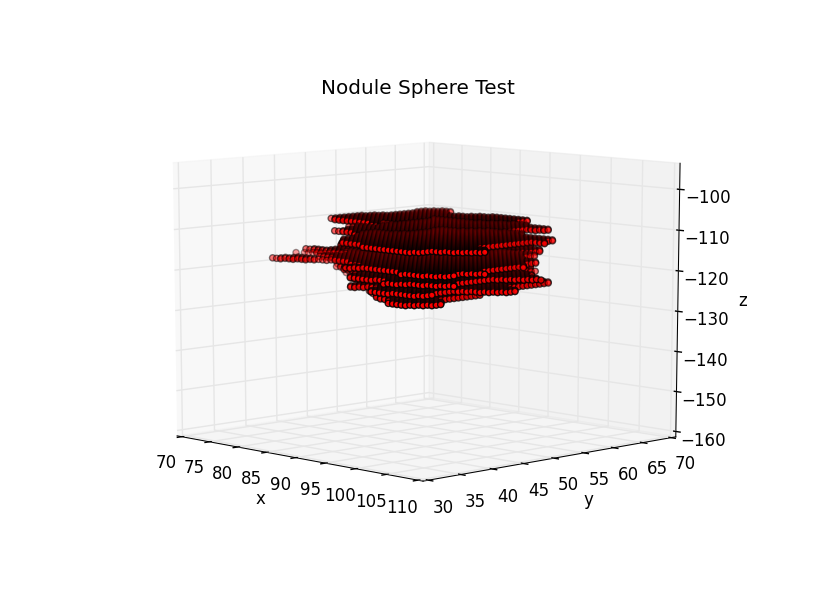
\includegraphics[width=90mm]{img/spherenodule_001.png}
    \caption{Flattened shape of nodule (LIDC scan 007)}
    \label{fig:flatNodule}
 \end{center}
\end{figure} %TODO use more LaTeX-friendly image format (pdf, eps)

To train a classifier, a list of positive and negative
examples are necessary. Therefore, a second list of voxels was constructed. The
amount of voxels was taken the same as in the list of positive voxels to obtain
a balanced traning dataset. The positions of the negative voxels were selected
at random over the entire image. The only constraint was that they were not
allowed the be situated within two times the maximum radius of each nodule. This
constraint was imposed to avoid ambigous training data.

Then features were calculated for both the positive and the negative voxels. The
features that were used are discussed in \ref{sec:featureExtraction}. This
resulted in a list of features and a class (nodule or non-nodule) per voxel.
This whole process was repeated for all scans and the results were then
concatenated to obtain a dataset to train the ensemble classifier.

\subsubsection{Feature extraction and selection} \label{sec:featureExtraction}
% TODO feature selection: empirisch
The \textbf{greyvalue} of each voxel was the only feature of the
cascaded classifier at level one. 
At level two two features were implemented: a blobdetector and a distance map
of the lung masks. The \textbf{blobdetector} was implemented as 
% TODO sven: Laplacians with different sigma values are applied on the remaining
% voxels + formule x =sqrt(2sigma)
% + uitleg welke sigma's -> statistieken

% TODO sven: uitleg distance map in 2 zinnen + fig


At the third and fourth level a \textbf{3D averaging method} \cite{keshani} was
implemented to get rid of the bronchi and bronchioles that were still not entirely eliminated. 

At a fifth level the \textbf{skewness and kurtosis} of a 3D window around each
voxel was calculated as a measure for the texture of a certain part of the image. The
skewness is a measure of the asymmetry of the probability distribution
distribution of a real-valued random variable (grey value) about its mean. The
kurtosis is a measure of the peakedness of the probability distribution of a
real-valued random variable. However, the implementation of these first order
statistics in the final classifier was prohibited by the time needed (hours) to
calculate these features for every voxel in the image.

% TODO subsectie
The rest of this paragraph provides an overview of other features that were
tested but that were not implemented in the final classifier because of several
reasons.

Another obvious feature, apart from the greyvalue of each voxel, is the
\textbf{position} $(X, Y, Z)$ of each voxel in the 3D image. An even better
feature is the \textbf{relative position} $(\tfrac{X}{X_{max}}, \tfrac{Y}{Y_{max}}, \tfrac{Z}{Z_{max}})$ as
it takes into account that the size of the datasets might change. However, after
testing it appeared that these features would only be useful if a very large
amount of training data was used. The training set had to be large enough so
almost every possible nodule position inside the lungs was covered by the
training data. As it is very difficult to estimate how many scans are needed for
this purpose and training on this large amount of data would take a lot of time,
the feature 'position' and 'relative position' were exluded from the featureset.
Instead a distance map based on the lung mask was implemented as a feature.

A \textbf{3D Sobel filter} for edge detection was implemented as well. A Sobel
filter is typically a $3 \times 3$ convolution mask that approximates the
partial derivative of an image along an axis. The results of multiple sobel
filters can be combined to calculate the gradient magnitude of each pixel. A
high magnitude usually corresponds with an edge in the original image.

To be really useful in nodule detection, the distance from each voxel to
neighbouring edges had to be calculated. However, due to a lack of time this was
not feasible anymore. Instead, the distance map mentioned above was used as a
substitute.

The \textbf{entropy} of an image is a measure for the chaos of the image in a
certain neighbourhood. Low entropy images are images where vast areas of pixels
have the same grey values. Images with high entropy show a large contrast
between neighbouring pixels. Therefore, it is a measure for the texture of an
image. The entropy of the entire 3D image was calculated and then the values for
each voxel were extracted. However, the time demand for these calculations were
far from negligible and as a consequence this feature was eliminated again.

A feature \textbf{neighbours} calculated the sum, the subtraction, the
multiplication and the quotient of the voxel in front and behind, left and right
and above and below a target voxel. Each of these operations where also
performed with the target voxel itself and the neighbouring voxel. Another
substantial amount of features were based on calculations within \textbf{3D
windows} that were swept over the lung mask of the image. The same operations
as in neighbours were executed on a larger scale: the neigbouring voxels were
determined by a certain adaptable window around the target voxel. Except for
these basic operations the mean, the standard variance, the minimum and the
maximum of the grey values of each window were calculated. Then these parameters
and the grey value of the target voxel were used for performing the basic
operations (sum, subtraction, multiplication, quotient) on. The same idea was
applied on the rows and columns in each window. The mean of different rows and
columns were determined and compared to each other by means of summing them up,
subtracting them, dividing one by another and multiplying them. In these windows
a frequency count was performed for each grey value in the window. These
frequencies were again compared. The results that were obtained this way could
be compared to one another by comparing the results for subwindows within larger
windows or within the entire image. However, none of these features were
implemented in the final classifier as calculating features for each individual
voxel in an image took too much time (hours).

\subsubsection{Training of the classifier}
\begin{algorithm}[H]
	\DontPrintSemicolon
	\caption{Training Phase\label{alg:train}}
	\ForEach{$dataset \in folder$}{
		load DICOM files\;
		load XML annotations\;
		\ForEach{$nodule \in annotations$}{
			\ForEach{$slice \in nodule$}{
				select positive voxels ($d < 0.66R_{min}$)
			}
		}
		\While {negative pixels $<$ positive pixels}
		{	select random pixel in volume\;
			\If{not near nodules ($d > 2R_{max}$)}{
				select negative voxel
			}
		}
	}
	\For{level from 1 to max}{
		\ForEach{selected pixel}{
			generate feature vectors up to level\;
		}
		train classifier\;
		save classifier model\;
	}
\end{algorithm}

\paragraph{Cross-validation}
During the training phase, we already want to get an idea about the future
performance of our classifier. Of course we could use the whole feature set in
the training, and use the same features afterwards to check if our classifier is
performing well. However, this is considered a form of cheating, and the test
would not tell us much about the predictive power of the classifier on new data.
That is why it is important to reserve a fraction of the feature vectors for
cross-validation. A strategy called stratified K-fold is used to repeatedly
split the feature set randomly in a train and a test fraction.
The stratified adjective means that the proportion of nodules to non-nodules are
similar in both fractions. Each time -- also called \textit{fold} -- the
classifier is trained with the train fraction and performance is checked with
the test fraction. After a number of folds, these results are combined to give a
proper estimate of the classifier performance in terms of accuracy (or other
score metric).

\subsection{Testing and validation of the classifier}
The model that was generated in the previous step is now applied on new data
to estimate the value of the added feature in the next level of the
classifier.
The question we ask ourselves here is whether a substantial amount of
non-nodule voxels are again removed from the dataset without removing the nodule
voxels as well. If this is the case the feature is kept at that level, otherwise
another feature is implemented.

The assessment is performed based on a probability image that is generated after
the model is applied on the new dataset. For each voxel in this dataset a
feature vector is calculated and this feature vector is then pushed down the
trees of the RF classifier. After each voxel is given a certain probability, the
probability image is generated.

\begin{algorithm}[H]
	\DontPrintSemicolon
	\caption{Testing \& Validation Phase\label{alg:test}}
	\ForEach{$dataset \in folder$}{
		load DICOM files\;
		mask $\longleftarrow$ load lung mask\;
		\For{level from 1 to max}{
			load classifier model\;
			\ForEach{$pixel \in mask$}{
				generate feature vector\;
				probability $\longleftarrow$ classify\;
			}
			combine into probability image\;
			mask $\longleftarrow$ (probability image $>$ cascade threshold)\;
		}
		discard non-nodule voxels ($p < 50$\%)\;
		cluster remaining voxels\;
		load XML annotations\;
		\ForEach{$nodule \in annotations$}{
			\eIf{any cluster $\in$ nodule ($d < 1.5R_{max}$)}{
				$TP{+}{+}$\tcc*[r]{nodule detected}
				delete clusters\;
			}{
				$FN{+}{+}$\tcc*[r]{nodule not detected}
			}
		}
		\ForEach{remaining cluster}{
			$FP{+}{+}$\tcc*[r]{spurious cluster}
		}
		calculate statistics
	}
\end{algorithm}

klassendiagram: hoe is programma opgebouwd?
TRAINING + TEST
\begin{enumerate}
\item stappen die doorlopen worden + fig
\item welke algorithmes gebruikt + wat doen ze + waarom die keuze?
\item vergelijken keuzes met literatuur/commerciele systemen?
\end{enumerate}


trainingstage + teststage
tussenresultaten: moeilijkheden, opl, \ldots




\section{TODO}
\begin{algorithm}[H]
	\DontPrintSemicolon
	\caption{Training Phase\label{alg:train}}
	\ForEach{$dataset \in folder$}{
		load DICOM files\;
		load XML annotations\;
		\ForEach{$nodule \in annotations$}{
			\ForEach{$slice \in nodule$}{
				select positive voxels ($d < 0.66R_{min}$)
			}
		}
		\While {negative pixels $<$ positive pixels}
		{	select random pixel in volume\;
			\If{not too close to any nodule}{
				select negative voxel
			}
		}
	}
	\ForEach{selected pixel}{
		\For{level from 1 to max level}{
			generate feature vector up to level\;
			train classifier\;
			save classifier model\;
		}
	}
\end{algorithm}

\begin{algorithm}[H]
	\DontPrintSemicolon
	\caption{Testing \& Validation Phase\label{alg:test}}
	\ForEach{$dataset \in folder$}{
		load DICOM files\;
		mask $\longleftarrow$ load lung mask\;
		\For{level from 1 to max level}{
			load classifier model\;
			\ForEach{$pixel \in mask$}{
				generate feature vector\;
				probability $\longleftarrow$ classify\;
			}
			combine into probability image\;
			mask $\longleftarrow$ (probability image $>$ cascade threshold)\;
		}
		discard non-nodule voxels ($p < 50$\%)\;
		cluster remaining voxels\;
		load XML annotations\;
		\ForEach{$nodule \in annotations$}{
			\eIf{any cluster $\in$ nodule ($d < 2R_{min}$)}{
				$TP++$\tcc*[r]{nodule detected}
				delete cluster\;
			}{
				$FN++$\tcc*[r]{nodule not detected}
				delete cluster\;
			}
		}
		\ForEach{remaining cluster}{
			$FP++$\tcc*[r]{spurious cluster}
		}
		calculate statistics
	}
\end{algorithm}

\subsection{Statistical Measurements}
In order to evaluate the performance of a binary classifier, we introduce some
statistical concepts. The reader should be familiar with Type I and Type II
errors. A Type I error occurs when the model predicts something to be there
while in reality it is not. In this text we call these occurences false
positives (FP). In our scenario, this corresponds with a classifier indicating
that a nodule is present when there is really none.

Vice versa, a Type II error occurs when the model predicts somethig to be absent
when in reality it present. We call them false negatives (FN). False negatives
in our scenario represent nodules not detected by the classifier.

Of course the classifier does not always have to be wrong. True positives (TP)
and true negatives (TN) respresent the cases where the classifier properly
detected the presence or absence of the nodule respectively.


\autoref{tbl:stats} summarizes these definitions.
\begin{table}[htp]
\begin{center}
	\begin{tabular}{r | c c}
						& Nodule 	& Non-Nodule \\
		    \hline
		    Positive 	& TP 		& FP\\
		    Negative 	& FN 		& TN \\
	\end{tabular}
	\caption{Summary of some basic statistical measures.}
	\label{tbl:stats}
\end{center}
\end{table}

Because the terms above are in absolute numbers, they are difficult to compare
across studies. That is where sensitivity and specifictiy come in. Sensitivity
compares the amount of true positives with the total amount of positives.
Synonyms include the true positive rate or the recall rate. Specificity does the
same for the negatives. It's sometimes also called true negative rate.

\begin{equation}
	sensitivity = \frac{TP}{TP + FP}
\end{equation}

\begin{equation}
	specificity = \frac{TN}{TN + FN}
\end{equation}

Ideally both measures should be 100\%, but that is an unrealistic expectation.
There is also an inherent trade-off between the two: when the sensitivity is
increased to make sure no false positives are detected, this will also increase
the false negatives, which in turn lowers specificity. In our case there is a
clear preference for a higher sensitivity, even though it may cost us some
specificity.

One last important measure is the accuracy. It is the ratio of all correctly
classified occurrences over all occurrences.

\begin{equation}
	accuracy = \frac{TP + TN}{TP + FP + TN + FN}
\end{equation}

%TODO voxels vs clusters vs nodules

\subsection{Laplacian}
One common feature in nodule detection is the laplacian -- also called blob
detector. The laplacian operator applied to a continuous 3D function is
defined as:

\begin{equation}
	\nabla^2f(x,y,z) = \left(\frac{\partial^2 f}{\partial x^2} + \frac{\partial^2
	f}{\partial y^2} + \frac{\partial^2 f}{\partial z^2}\right)
\end{equation}

To be applied to images, it must first be discretized into a 3D convolution
mask. That mask typically has a large negative number in the center, surrounded
by positive ones.

However, because we are dealing with second derivatives, this operation is very
sensitive to noise. One solution to this problem is to convolve the image with a
gaussian kernel first. Because this kernel has a low-pass effect, noise will be
reduced.

\begin{equation}
	g(x,y,z;t) = \frac{1}{(\sqrt{2\pi} t)^3}e^{-\frac{x^2+y^2+z^2}{2t^2}}
\end{equation}

It can be represented by bionomial filters -- repeated convolutions for [1 1]
with itself -- in the discrete domain, making it rather cheap operation
compution-wise.

Convolution has some interesting properties, which allow this calculation to be
further optimized:

\begin{equation}
	\nabla^2(g * f) = (\nabla^2 g) * f %TODO continue
\end{equation}

Alternatively to the Laplacian, one can also use the Hessian matrix of second
partial derivatives as a feature. The laplacian is simply the sum of the
elements on the main diagonal. In that sense it is more complete, but also much
more computationally expensive. For this reason, we stick with the laplacian
operator.


\subsection{Cross-validation}
During the training phase, we already want to get an idea about the future
performance of our classifier. Of course we could use the whole feature set in
the training, and use the same features afterwards to check if our classifier is
performing well. However, this is considered a form of cheating, and the test
would not tell us much about the predictive power of the classifier on new data.
That is why it is important to reserve a fraction of the feature vectors for
cross-validation. A strategy called stratified K-fold is used to repeatedly
split the feature set randomly in a train and a test fraction.
The stratified adjective means that the proportion of nodules to non-nodules are
similar in both fractions. Each time -- also called \textit{fold} -- the
classifier is trained with the train fraction and performance is checked with
the test fraction. After a number of folds, these results are combined to give a
proper estimate of the classifier performance in terms of accuracy (or other
score metric).

\section{Results and discussion}
\subsection{Optimisation of the classifier parameters}
By performing a five fold cross validation during the training stage the most
optimal parameter set for the RF algorithm were discovered. It was found that
for all levels except the first, a value of 5 yields optimal results for the
minimum samples per leaf parameter. For level 1, this optimal value was
significantly higher at 55. This makes sense as higher values correspond to less
complex classifiers.

The accuracy that was reached was respectively 80,5\%, 97,9\%, 98,1\% and 98,2\%
for the four consecutive levels. This shows that the first two levels in the
cascade contributed more in the process of removing negative voxels the the two
last levels. The latter however were not useless as they still increased the
level of accuracy. The fourth level for example still eliminated about 600
voxels per scan. Though, as mentioned before, the accuracy metric should be taken
with a grain of salt in highly unbalanced classification tasks.

For each level of the classifier a threshold was set to determine which voxels
would be allowed to the next level (i.e. which voxels showed a higher nodule
probability). In order to avoid discarding nodule voxels of small nodules a
rather low threshold had to be set. These were empirically determined at 20\%,
40\%, 40\% and 70\% for the four levels respectively, although more rigorous
testing might yield even better values.

\subsection{Validation results}
In this section, we will illustrate our results based on two slices from the
fiftieth LIDC dataset. The volume dimensions are $512 \times 512\times 139$ and
it contains one nodule around slice 95. As figure \ref{fig:d50} shows, slice 50
contains no nodules while slice 95 indeed contains exactly one. After applying
the lung mask, 13,59\% of all voxels remain.

\begin{figure}[ht]
\begin{center}
	\begin{subfigure}[b]{\linewidth}
		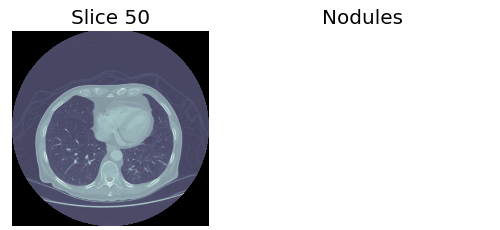
\includegraphics[width=\linewidth]{img/cascades/D50S50.png}
		\caption{Slice 50}
	\end{subfigure}
	\begin{subfigure}[b]{\linewidth}
		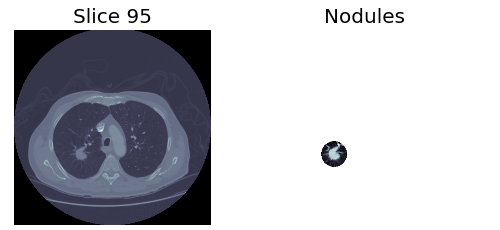
\includegraphics[width=\linewidth]{img/cascades/D50S95.png}
  		\caption{Slice 95}
	\end{subfigure}
	\caption{Example of two slices in dataset 50, one without and one with a
	nodule.}
	\label{fig:d50}
\end{center}
\end{figure}

\paragraph{Level 1}
As expected, we get a significant reduction in the number of voxels. More
specifically only soft tissue structures -- i.e. lung wall, bronchi/bronchioli
and nodules -- remain. The threshold performs a straightforward segmentation and
can not be improved much.

\begin{figure}[p]
\begin{center}
	\begin{subfigure}[b]{\linewidth}
		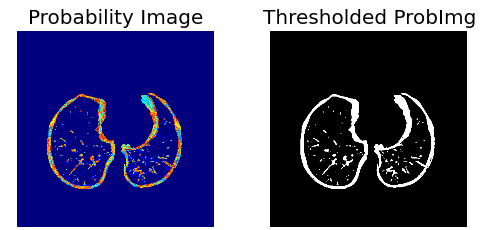
\includegraphics[width=\linewidth]{img/cascades/D50S50L1.png}
		\caption{Level 1 -- Threshold: 20\% -- 5,74\% remaining}
	\end{subfigure}
	\begin{subfigure}[b]{\linewidth}
		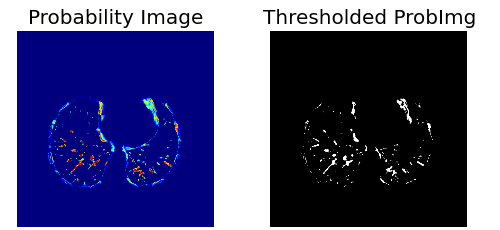
\includegraphics[width=\linewidth]{img/cascades/D50S50L2.png}
		\caption{Level 2 -- Threshold: 40\% -- 1,86\% remaining}
	\end{subfigure}
	\begin{subfigure}[b]{\linewidth}
		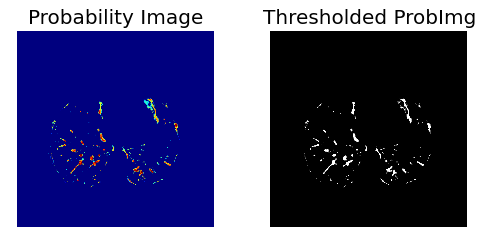
\includegraphics[width=\linewidth]{img/cascades/D50S50L3.png}
		\caption{Level 3 -- Threshold: 40\% -- 1,55\% remaining}
	\end{subfigure}
	\begin{subfigure}[b]{\linewidth}
		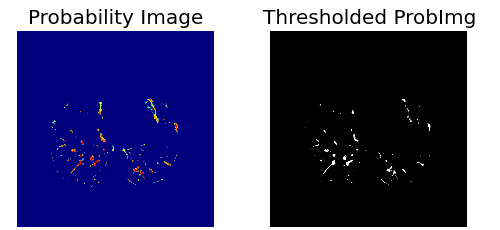
\includegraphics[width=\linewidth]{img/cascades/D50S50L4.png}
		\caption{Level 4 -- Threshold: 70\% -- 0,54\% remaining}
	\end{subfigure}
  \caption{Processed versions of slice 50 in dataset 50. Left: probability
  image. Right: threshold of probability image showing the voxels that continue
  to the next level in the cascade. The algorithm started with 13,59\% of all 
  voxels remaining after lung segmentation.}
  \label{fig:d50s50}
\end{center}
\end{figure}

\begin{figure}[p]
\begin{center}
	\begin{subfigure}[b]{\linewidth}
		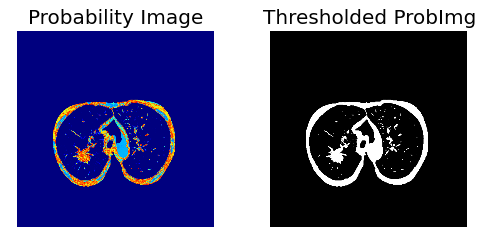
\includegraphics[width=\linewidth]{img/cascades/D50S95L1.png}
		\caption{Level 1}
	\end{subfigure}
	\begin{subfigure}[b]{\linewidth}
		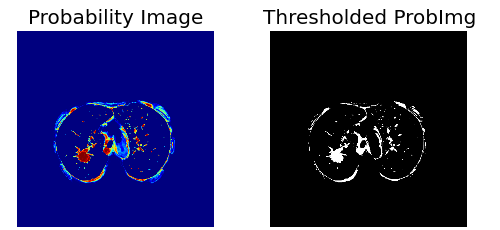
\includegraphics[width=\linewidth]{img/cascades/D50S95L2.png}
		\caption{Level 2}
	\end{subfigure}
	\begin{subfigure}[b]{\linewidth}
		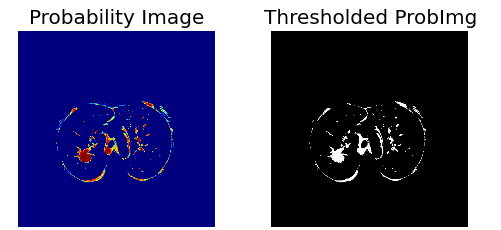
\includegraphics[width=\linewidth]{img/cascades/D50S95L3.png}
		\caption{Level 3}
	\end{subfigure}
	\begin{subfigure}[b]{\linewidth}
		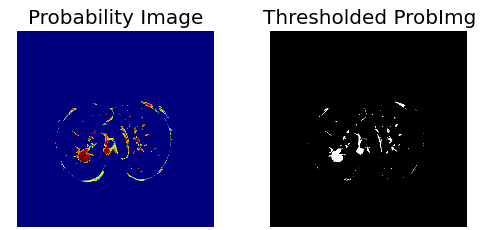
\includegraphics[width=\linewidth]{img/cascades/D50S95L4.png}
		\caption{Level 4}
	\end{subfigure}
  \caption{Processed versions of slice 95 in dataset 50. Left: probability
  image. Right: threshold of probability image showing the voxels that continue
  to the next level in the cascade. The same thresholds and remaining counts
  apply as in figure \ref{fig:d50s50}.}
  \label{fig:d50s95}
\end{center}
\end{figure}

\paragraph{Level 2}
This level was meant to highlight nodule-sized blobs while reducing the response
of other structures, in particular lung walls. The laplacian filter certainly
succeeded in the former, although we still get a medium-high response from
certain wall segments at times. Unfortunately, the laplacian also highlights the
smaller structures in the lung. This was inevitable as we needed LoG filters
with small sigmas to find small nodules. There is definitely room for
improvement in threshold level. A higher threshold could discard more wall
voxels while retaining nodules. In conclusion it is still a well performing
feature that significantly reduces the voxel count, although it has some
unfortunate side effects.

\paragraph{Level 3 and 4}
The goal here was to discriminate between small bronchioli and blood vessels on
the one hand, and small nodules on the other hand by means of 3D averaging.
Unfortunately, this feature does not perform as well as hoped: there is only a
margin decrease in non-nodule voxels. Note that the fourth level feature with
the larger internal threshold works slightly better, but still not satisfactory.
Future work should either fine-tune the parameters of this method or find a more
effective method altogether.

The obtained sensitivity of the algorithm was 100,00\% with an average of 2,17
TP and 4279,43 FP per scan. This high number of FP results a in very low
precision of 0,0634\%. Training the algorithm on 30 scans took 1 hour and 50
minutes. The processing of a new medium large dataset (136 slices) takes about
10 minutes.
% TODO FPs of FP?
Keeping in mind that comparing different studies is difficult (see section
\ref{sec:performance}), some relevant results from literature are presented
here. \cite{teramoto} used a cylindrical nodule-enhancement filter and performed
a FP reduction using a SVM classifier. This method reached a sensitivity of 80\%
and 4,2 FP per LIDC/IDRI scan. The detection speed was 25-34 seconds per scan.
\cite{elbaz} applied template matching and found a sensitivity of 82,3\% and a
specificity of 9,2\%. The time to process 1 scan in C++ was about 5 minutes.
\cite{lee2010} tested an ensemble classification aided by clustering (CAC)
method on a set of nodules and non-nodule examples and they obtained a
classification accuracy of 97,72\%. An execution time of 190 seconds was
registered.

These results indicate our algorithm performed well concerning detecting all
nodules, but the amount of FP has to be reduced to get the precision up. At the
moment, the algorithm is simply not strict enough: it detects all nodules but at
a high FP cost. This amount can be reduced in a first stage by determining
the optimal value for all parameters, such as the threshold for each cascade
level.

Our ``potential nodule'' clustering strategy also plays a significant role here.
By clustering individual voxels together we hope to make them more comparable
to nodules, but this is not always the case. Some clusters are simply too small
to even represent a realistic nodule. Filtering out these clusters will help
boost our results.

Another way of improving the algorithm is increasing the amount of training
data. To determine the optimal amount of datasets a trade-off should be made
between the time it takes to train the algorithm with extra datasets and the
diminishing marginal improvements in the performances of that action. 

A third possibility is implementing more features (e.g. haar features),
especially features focusing on removing edges and eliminating the bronchioles.
On the other hand, implementing more features will increase the processing time.
However, by optimising the thresholds in the existing algorithm these things can
also be (partially) achieved. The threshold on level can be set higher which
will remove more edges. For eliminating the bronchioles the parameters of the 3D
averaging features should be optimised. The results from the literature also
show that we have a long processing time. However, one has to take into account
that the implementation of this algorithm was done in Python -- an interpreted
language -- which makes it inherently slower than low-level compiled languages
such as C++. Nevertheless, Python was chosen for its rapid prototyping
abilities. Future work may implement our algorithm in C++ or another compiled
language to speed up the computational process.

\cite{ginneken} compared the performances of six nodule detection CAD algorithms
on the same validation dataset. The sensitivities at seven levels of false
positive detection were calculated and then averaged. The best performing method
in this study yielded an average sensitivity of 63,2\% for the detection of all
kinds of nodules. The sensitivity per nodule type was also provided: small
nodules (63,4\%), large nodules (62,8\%), isolated nodules (60,9\%), vascular
nodules (69,3\%), pleural nodules (43,5\%) and peri-fissural nodules (76,6\%).
This clearly shows that the ease of nodule detection also depends on the type of
nodule. As this information is not available in the annotations of the scans and
as we did not cooperate with a radiologist, it is not possible to differentiate
between the different types of nodules in this project. However, as we may
assume that different nodule types are represented in our testset, it is clear
the algorithm is able to detect several types of nodules except for extremely
small ones as we removed these from the annotations in the training and
validation phase.

%TODO suggest using cross validation for the 30-8 groups as well

\section{Conclusion}
CT technology has come to the point where high resolution images of the whole
chest can be obtained in a single breath hold. The resolution allows to detect
pulmonary nodules in an early stage and therefore CT scans become more and more
part of routine investigations. This causes a large increase in the workload of
the radiologists, who are only human and thus also prone to errors. Time
pressure and fatigue may lead to an increasing fraction of overlooked nodules.
Research showed however that pulmonary lung detection systems, that serve as a
second reader, can improve the performances of radiologists.
Therefore, the goal of this project was to develop an accurate, fast and
automated system to detect pulmonary nodules in CT scans.

A non-exhaustive literature review revealed that companies such as R2
Technology, Siemens, iCAD etc. already have invested in the development of
similar software. However, a satisfying allround software package does not exist
yet. The research is still ongoing to develop a system with 100\% sensitivity
and no false positives detection. One of the problems that arises here is that
there is no golden standard to measure the performance of the CAD system
against. Currently, the performances of CAD systems are compared with the
findings of one or more radiologists. Although the fraction of overlooked
nodules decreases when more radiologists cooperate when analysing a CT scan,
there is no guarantee that all nodules are delineated in a scan. This makes it
very hard to assess the performance of a automated nodule detection system.

There are three main schools of thought in the development of pulmonary nodule CAD
systems. The first group uses template matching to detect (a type of) nodules. A
second group performs a nodule segmentation by means of a series of
morphological operations, active contour modelling, etc. The third group applies
classification methods, possibly aided by clustering. As there is evidence
in literature that this method yields the best results, a more extensive
literature review was performed to select a proper classification method. It was
decided to use a cascaded Random Forest classifier as this type of classifiers
is not yet fully explored in this area of research. This provided the
opportunity to beat the state of the art in nodule detection algorithms.

Random Forests have many advantages. As an ensemble classifier it combines
decisions of multiple classifiers to form an integrated output. This way of
working has the advantage that a better predictive performance is obtained
compared to the predictive performance demonstrated by each individual learning
algorithm separately. Furthermore, Random Forests are rather robust against
noise compared with other classifier such as Support Vector Machines. Random
Forests also allow to use a lot of features, even if they have different orders
of magnitude, without increasing the time complexity too much. The features also
do not have to be known in advance. At the same time, the method does not
require a lot of parameter tuning. The only thing that has to be taken into
consideration is the depth of the trees as overfitting must be avoided in order
to maintain an algorithm that is able to generalise across datasets. The use of
a cascaded classifier is preferred as it limits the amount of CPU time and
memory storage.
 
The higher the level in the cascaded classifier, the more complex the features.
On the first level the grey values of the voxels were used to detect soft
tissue, to which class nodules belong. Although this first level is able to
eliminate the voxels outside the lungs, a lung segmentation was applied first to
reduce the amount of voxels to be processed. The reason for this were recurrent
memory errors when attempted otherwise. On the second level a blobdetector --
Laplacian filter -- and a distance map were implemented. On the third and fourth
level a 3D averaging algorithm was elaborated with two different
parametersettings. This 3D averaging allows to separate nodules from bronchioles
and bronchi by taking into account the presence of these structures in the
preceeding and/or succeeding slices. A lot of other features were implemented
and tested, but most of them were removed again from the final classifier as
they required a lot of processing time and did not perform accordingly. After
each level in the classifier a threshold was set to determine which voxels were
taken to the next level and which were to be discarded. These thresholds were
empirically determined, but can still be optimised. The training and the
validation of the algorithm were performed on 30 and 8 datasets respectively.

During the training of the algorithm a five-fold crossvalidation was performed
to determine the optimal set of parameters for the Random Forest algorithm. It
was decided to take into account the optimal number of minimum samples per leaf
to keep the algorithm from overfitting. An accuracy level of 98,2\% was achieved
in the last level of the cascaded classifier.

The validation of the optimised classifier showed 100\% sensitivity, but also
indicated the amount of false positives still has to be significantly reduced.
The processing time of 10 minutes per scan is not extremely satisfying, but one
has to take into account that Python is an interpreted language which makes it
inherently slower than for instance C++. Transferring the code to a compiled
language will speed up the process. The aim is to be able to process one scan
within a few minutes. There is no need for faster processing as a radiologist
will not need the results earlier, but it should not take much longer either.

The amount of false positives per scan (4279,43 FP per scan) has to be reduced.
A first step to achieve this is the optimisation of the thresholds in the
algorithm. A more accurate setting of the thresholds will also be possible if the
algorithm is trained on a larger amount of scans. On top of that, the clustering
strategy might have to be revisited. Another possibility is the implementation
of more features. However, there are two constraints here. The first
one is trivial: the more features, the longer it will take to process the scan.
A second consideration that has to be made is the fact that not all features are
suitable for our approach. We only selected features that could be extracted
from the image without performing any nodule segmentation in advance to make the
algorithm faster an more robust. This nodule segmentation step would allow to
use a wider range of features, but could also introduce errors in the algorithm.
Furthermore, developing a nodule segmentation is not a trivial thing to do.

Although the use of the features and the code of the cascaded classifier were
optimised considerably, one of the largest problems we encountered were the
recurring out-of-memory errors. In the beginning of the project we decided to
use Python 2.7.6 in the 32-bit version as it is typically more stable than the
64-bit version. This showed to be a bad choice later on as we had to spend a lot
of time and efforts on the optimisation of the code concerning memory storage
and computational power. This also prevented us from implementing a lot of
features as we intended to do. The first concept was to calculate a range of
features and let the Random Forest algorithm then decide on which and how many
features to use in the final classifier. Because of the memory errors, we had to
carefully select the features ourselves by visual assessment of the probability
images that were generated at each level in the classifier, rather than letting
RF figure out the most interesting features from a large pool.

Some other things to be done differently in the future is limiting the amount
of time spent on reviewing the literature, limiting the amount of time spent
on optimising the threshold values and performing the implementation of the
features in a different way. In the beginning of the project we implemented a
lot of features, which was also the aim before we encountered the memory
errors, but a lot of them proved to be useless or required too much processing
time. Instead, we should have tried some features, trained the algorithm and
make decisions on the type and amount of feautures based on these small
experiments.

Besides the suggestions for improvement mentioned above, we have some other
recommendations for future research. First of all, it would be interesting to
not only detect the nodules, but also classify them as benign or malignant. In
order to do this the grey value intensity gradient inside the nodule could be a
helpful feature. In order to implement this feature, the nodule voxels should be
clustered first. Also classifying the nodules accoring to the type of nodule
(juxta-vascular; pleural tail; well-circumscribed; juxta-pleural) would be
interesing as the type may already be an indication for the probability of
malignancy of a nodule. As the type of nodule was not available in the
annotations, it was not possible for us to implement this in the classifier.
An interesting comparison that can be made is whether the subtelty
that is assigned by the radiologist is comparible with the probability provided
by the algorithm. And may the algorithm overlook the same nodules as one
radiologist when assessing the CT scan?

Finally, if all optimalisations are performed the algorithm can be implemented
in MeVisLab as a stand-alone modules which can easily be used by radiologists or
researchers. To assess the performance of the optimised algorithm it can be
validated on the dataset of the ANODE09 challenge where it can be compared with
the results of other studies.

\clearpage
\appendix
\section{Appendix}
\subsection{Meetings}
%
\includepdf[pages={-}]{meetings/1.pdf}
%
\includepdf[pages={-}]{meetings/2.pdf}
%
\includepdf[pages={-}]{meetings/3.pdf}
%
\includepdf[pages={-}]{meetings/4.pdf}
%
\includepdf[pages={-}]{meetings/5.pdf}
%
\includepdf[pages={-}]{meetings/6.pdf}
%
\includepdf[pages={-}]{meetings/7.pdf}
%TODO include logbook
%TODO include mission definition

\clearpage
\bibliographystyle{alpha} %plain,unsrt,alpha,abbrv,acm,apalike,siam,ieeetr,..
\bibliography{references}
\end{document}